\subsection{Propriedades da Entropia}
\begin{frame}%[allowframebreaks]
  \frametitle{Propriedades da Entropia}
  \begin{enumerate}
    \item $H$ é uma função estritamente côncava de $X$, i.e., para $0 \leq \lambda \leq 1$
      e variáveis aleatórias $X$ e $Y$
      \begin{equation}
        H(\lambda X + (1 - \lambda) Y) \geq \lambda H(X) + (1 - \lambda) H(Y)
      \end{equation}
      com igualdade sse (se e somente se) $\lambda = 0$ ou $\lambda = 1$ ou $X=Y$.
    \item $H(X) \geq 0$ com igualdade sse $p(X)$ for não nulo apenas em um ponto $x_0 \in \mathcal{X}$.
    \item $H(X) \leq \log \vert \mathcal{X} \vert$ com igualdade sse $p(X)$ for uniforme ($p \sim \frac{1}{n}$).
    \item $H(X)$ é uma função apenas das probabilidades $p(x_i)$, independente da ordem ou rótulo.
    \item $H_b(X) = (\log_b a) H_a(X)$.
  \end{enumerate}
\end{frame}


\subsection{Continuidade da Entropia}
\begin{frame}[allowframebreaks]
  \frametitle{Continuidade da Entropia}

  Todas as medidas de informação de Shannon são funções contínuas das distribuições
  conjuntas das variáveis aleatórias envolvidas.

  \begin{definition}[distância das variações]
  Seja $p$ e $q$ duas distribuições probabilísticas em um alfabeto comum $\mathcal{X}$.
  A distância das variações entre $p$ e $q$ é definida por
  \begin{equation}
  V(p,q) = \sum_{x \in \mathcal{X}} \vert p(x) - q(x) \vert .
  \end{equation}
  \end{definition} 

  Dado um alfabeto finito fixo $\mathcal{X}$, considere $\mathcal{P}_\mathcal{X}$ o
  conjunto de todas as distribuições em $\mathcal{X}$. A entropia para uma dada distribuição
  $p$ sobre o alfabeto $\mathcal{X}$ é definida por
  \begin{equation}
  H(p) = - \sum_{x \in S_p} p(x) \log p(x) ,
  \end{equation}
  onde $S_p$ denota o suporte de $p$, ou seja, $S_p \subset \mathcal{X}$.
  
  Para que $H(p)$ seja contínuo com respeito à convergência em distância das variações,
  em uma determinada distribuição $p \in \mathcal{P}_\mathcal{X}$, devemos ter que,
  para qualquer $\epsilon > 0$, existe $\delta > 0$ tal que
  \begin{equation}
  \vert H(p) - H(q) \vert < \epsilon ,
  \end{equation}
  para todo $q \in \mathcal{P}_\mathcal{X}$ satisfazendo 
  \begin{equation}
  V(p,q) < \delta ,
  \end{equation}
  ou, de forma equivalente, 
  \begin{equation}
  \lim_{p' \rightarrow p} H(p') = H\left( \lim_{p' \rightarrow p} p' \right) = H(p) ,
  \end{equation}
  onde a convergência $p' \rightarrow p$ é em distância das variações.

  Como $a \log a \rightarrow 0$ quando $a \rightarrow 0$, definimos uma função 
  $l:[0,\infty) \rightarrow \mathbb{R}$ da forma
  \begin{equation}
  l(a) = \begin{cases} 
        a\log a & \quad \text{se } a > 0 , \\
        0       & \quad \text{se } a = 0 ,
        \end{cases}
  \end{equation}
  ou seja, $l(a)$ é uma extensão contínua de $a \log a$.
  Podemos reescrever a entropia da seguinte forma
  \begin{equation}
  H(p) = - \sum_{x \in \mathcal{X}} l(p(x)) ,
  \end{equation}
  onde o somatório é tomado em todo $x \in \mathcal{X}$ ao invés de $S_p$.
  Definindo uma função $l_x: \mathcal{P}_\mathcal{X} \rightarrow \mathbb{R}$, para
  todo $x \in \mathcal{X}$, da forma 
  \begin{equation}
  l_x(p) = l(p(x)) ,
  \end{equation}
  teremos
  \begin{equation}
  H(p) = - \sum_{x \in \mathcal{X}} l_x(p) . \label{eqHsumXl}
  \end{equation}
  Evidentemente $l_x(p)$ é contínua em $p$ (com relação à convergência em 
  distância das variações). Como o somatório na Equação \ref{eqHsumXl} possui
  apenas um número finito de termos, podemos concluir que $H(p)$ é uma função
  contínua de $p$.
\end{frame}


\subsection{Limite Superior da Entropia}
\begin{frame}%[allowframebreaks]
  \frametitle{Limite superior para o Log} 
  \begin{figure}[h!]
  \centering
  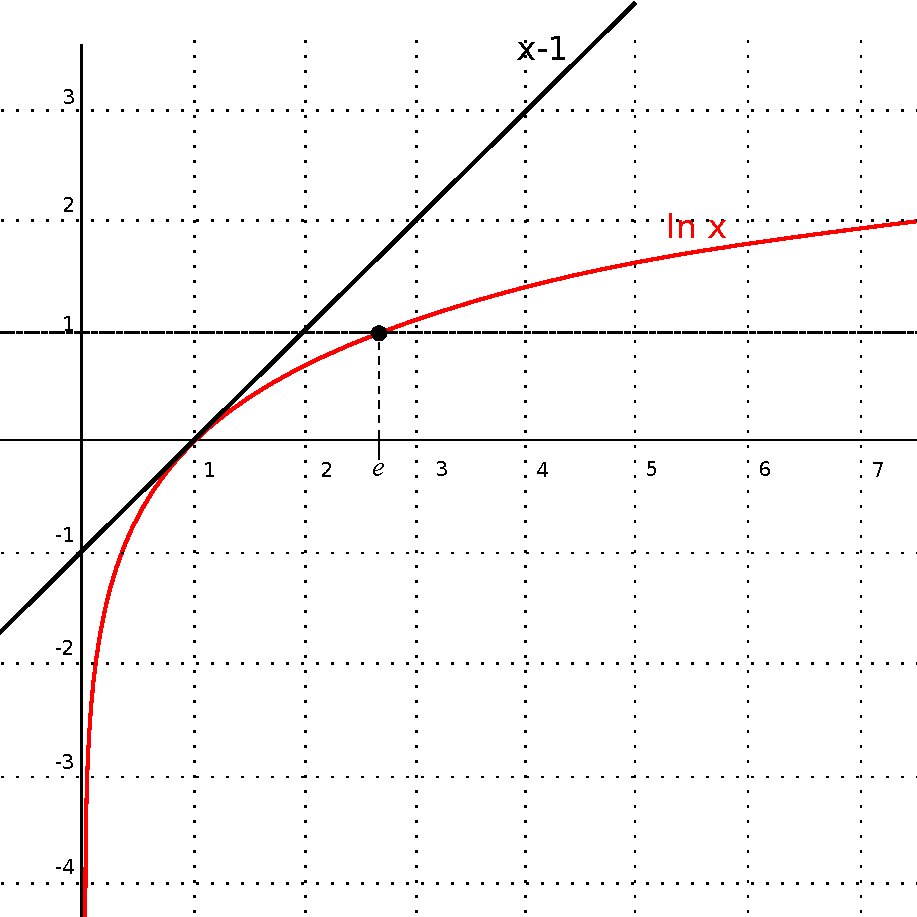
\includegraphics[width=0.4\textwidth]{images/lnx-x-1.pdf}
  %\caption{.}
  \label{fig:lnx-x-1}
  \end{figure}
  \begin{equation}
  \ln x \leq x-1
  \end{equation}
\end{frame}
\note{
$\ln x \leq x-1$, para $x \geq 1$

\begin{itemize}
\item Sabemos que para $x=1$ é verdadeiro, $0 = \ln 1 \leq 1 - 1 =0$.
\item Vamos demonstrar que $\ln x \leq x-1$, para $x \geq 1$ por contradição.
\end{itemize}
Suponha que existe $b > 1$ tal que $\ln x > x - 1$, para $x=b$.
Vamos definir $f(x) = \ln x - x + 1$, logo $f(1) = 0$ (conforme visto acima)
e $f(b) > 0$ (por hipótese).
Pelo teorema do valor médio $\exists c$, $1 < c < b$, tal que
\begin{equation}
f'(c) = \frac{f(b) - f(1)}{b - 1} = \frac{\overbrace{f(b)}^{>0}}{\underbrace{b-1}_{>0}} > 0 .
\end{equation}
Mas, $f'(x) = 1/x -1$, e assim $f'(x) < 0$ para $x>1$. Logo há uma contradição
e nossa hipótese é falsa. Teremos assim $\ln x \leq x-1$, para $x \geq 1$.

Para $x \in (0,1)$, basta seguir os mesmos passos, escolhendo um ponto 
$x=b$, tal que $0 < b < 1$. Vamos encontrar um ponto $c$ tal que $0 < b < c < 1$. 
E usar o teorema do valor médio para mostrar uma contradição na hipótese.  
}


\begin{frame}[allowframebreaks]
  \frametitle{Valor Máximo da Entropia (discreta)}
  \begin{theorem}[Limite Superior da Entropia]
  Seja $X \in \{x_1, x_2, \ldots, x_n\}$. Então $H(X) \leq \log n$, sendo a igualdade
  alcançada se e somente se $p(X=x_i) = \frac{1}{n}$ para todo $i$. 
  \end{theorem}
  \framebreak
  \begin{proof}
  Vamos mostrar que $H(X) - \log n  \leq 0$.
    \begin{eqnarray}
    H(X) - \log n &=& - \sum_x p(x) \log p(x)  - \log n \overbrace{\sum_x p(x)}^{=1} \nonumber \\
        &=& - \sum_x p(x) \log p(x) - \sum_x p(x) \log n \nonumber \\
        &=& - \sum_x p(x) \log p(x) n = \log_2 e \sum_x p(x) \ln \frac{1}{p(x) n} \nonumber \\
        &\leq& \log_2 e \sum_x p(x) \left[ \frac{1}{p(x) n} -1 \right] \nonumber
    \end{eqnarray}

   \proofbreak
    \begin{eqnarray}
    H(X) - \log n &\leq& \ldots \nonumber \\
        &=& \log_2 e \left[ \underbrace{\sum_x \frac{1}{n}}_{\sum_{x \in \mathcal{X}} \frac{1}{n} = n \frac{1}{n} = 1} - \underbrace{\sum_x p(x)}_{=1} \right] = 0
    \end{eqnarray} 
  \end{proof} 
\end{frame}


\begin{frame}%[allowframebreaks]
  \frametitle{Valor Máximo da Entropia}
  Na demonstração acima utilizamos $\ln z \leq z - 1$. A igualdade $\ln z = z-1$ se dará
  no ponto estacionário $z=1$, isto é, quando $\frac{1}{p(x) n} = 1$, ou seja,
  quando $p(x) = 1/n$, teremos assim uma distribuição uniforme.

  \vspace{1cm}
  Se tivermos $p_i = 1/n$, então
  \begin{equation}
  - \sum_i p_i \log p_i = - \sum_i \frac{1}{n} \log \frac{1}{n} = - \log \frac{1}{n} = \log n .
  \end{equation}
  Podemos mostrar (através da concavidade da entropia) que este é o único conjunto de valores com esta propriedade.

  \begin{itemize}
  \item Entropia aumenta quando a distribuição se torna mais uniforme.
  \end{itemize}
\end{frame}

\begin{frame}[allowframebreaks]
  \frametitle{Valor Máximo da Entropia}
  Outra demonstração...

  \begin{proof}
    Considere $X \in \mathcal{X} = \{x_1, x_2, \ldots, x_n\}$ com probabilidades
    $p=\{p_1, p_2, \ldots, p_n\}$, respectivamente. A entropia de $X$ é dada por
    \begin{eqnarray}\label{eq-dem-entr-max2}
    H(X) &=& - \sum_{i=1}^n p_i \log p_i \nonumber \\
        &=& - \sum_{i=1}^{n-1} p_i \log p_i - p_n \log p_n \nonumber \\
        &=& - \left( \frac{1}{\ln 2} \right) \left[ \sum_{i=1}^{n-1} p_i \ln p_i + p_n \ln p_n \right] .
    \end{eqnarray}
    \proofbreak

    Da mesma forma, podemos expressa $p_n$ da seguinte maneira
    \begin{equation}\label{eq-pn-n-1}
    p_n = 1 - \sum_{i=1}^{n-1} p_i .
    \end{equation}
    Utilizando \ref{eq-pn-n-1} em \ref{eq-dem-entr-max2}, podemos expressar
    a entropia $H(X)$ como uma função de $n-1$ probabilidades $p_i$. O máximo
    será dado quando a seguinte condição ocorrer
    \begin{equation}\label{eq:condmaxent}
    \frac{\partial H(X)}{ \partial p_k } = 0 \textmd{ \ for \ } k = 1, \ldots, n-1 \textmd{ .}
    \end{equation}

    \proofbreak
    Teremos então
    \begin{eqnarray}\label{ea:dHeqz}
        0 = \frac{\partial H(X)}{ \partial p_k } &=&  - \left( \frac{1}{\ln 2} \right) \frac{\partial}{ \partial p_k } \left[ \sum_{i=1}^{n-1} p_i \ln p_i  + p_n \ln p_n \right] \nonumber \\
        &=& - \left( \frac{1}{\ln 2} \right) \left[ \ln p_k + 1 + (\ln p_n + 1) \frac{\partial p_n}{ \partial p_k }  \right] \nonumber \\
        &=& - \left( \frac{1}{\ln 2} \right) \left[ \ln p_k + 1 - (\ln p_n + 1) \right] ,
    \end{eqnarray}
    onde utilizamos a Equação \ref{eq-pn-n-1}, que nos fornece $\partial p_n / \partial p_k = -1$.

    \proofbreak
    A Equação \ref{ea:dHeqz} mostra que devemos encontrar $\ln p_k = \ln p_n$ para cada $k=1,\ldots,n-1$.
    Todas as $n-1$ equações serão satisfeitas quando todas as probabilidades $p_k$ forem iguais a $1/n$.

    \proofbreak
    Devemos agora calcular a derivada segunda para mostrar que o extremo que achamos é de fato um máximo.
    \begin{eqnarray}\label{ea:d2Heqz}
        \frac{\partial^2 H(X)}{ \partial p_k^2 } &=& - \left( \frac{1}{\ln 2} \right) \frac{\partial}{ \partial p_k } \left[ \ln p_k - \ln p_n \right] \nonumber \\
           &=& - \left( \frac{1}{\ln 2} \right) \left[ \frac{1}{p_k} + \frac{1}{p_n} \right] \leq 0 \textmd{ ,}
    \end{eqnarray}
    já que as probabilidades são valores positivos. Escolhendo então $p_k = 1/n$, teremos a entropia máxima.

  \end{proof}
\end{frame}



\subsection{Subdividindo em partes}
\begin{frame}[allowframebreaks]
  \frametitle{Subdividindo a entropia em partes}
  A entropia deve permanecer inalterada, mesmo quando subdividimos as escolhas em partes.
 
  \begin{example}[Exemplo simples]
  Suponha uma v.a. $X$ com alfabeto $\mathcal{X} = \{x_1, x_2, x_3, x_4 \}$
  e distribuição $q = (q_1. q_2, q_3, q_4)$.

  A entropia associada a esta variável aleatória é dada por
  \begin{eqnarray}
  H(X) &=& H(q_1, q_2, q_3, q_4) \nonumber \\
        &=& - \sum_{i=1}^{4} q_i \log q_i \nonumber \\
        &=& - q_1 \log q_1 - q_2 \log q_2 - q_3 \log q_3  - q_4 \log q_4 .
  \end{eqnarray}

  \examplebreak

  Se dividirmos a escolha na determinação de $X$ em duas escolhas sucessivas,
  conforme ilustrado na figura abaixo, poderemos então escrever
  \begin{equation}
  H(q_1, q_2, q_3, q_4) = H(p_1, p_2) + p_1 H(p_{1,1}, p_{1,2}) + p_2 H(p_{2,1},p_{2,2}) .
  \end{equation}

        \begin{figure}[h!]
        \centering
        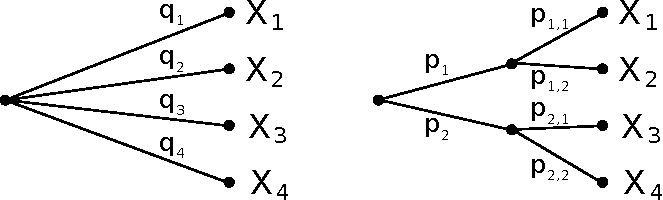
\includegraphics[width=0.5\textwidth]{images/choices4.pdf}
        \label{fig:choices4}
        \end{figure}

  \examplebreak
  \vspace{-2ex}
  \begin{eqnarray}
  H(X)  &=& - q_1 \log q_1 - q_2 \log q_2 - q_3 \log q_3  - q_4 \log q_4 \nonumber \\
        &=& - p_1 p_{1,1} \log p_1 p_{1,1} - p_1 p_{1,2} \log p_1 p_{1,2} - p_2 p_{2,1} \log p_2 p_{2,1} - p_2 p_{2,2} \log p_2 p_{2,2} \nonumber \\
        &=& - p_1 p_{1,1} \log p_1 - p_1 p_{1,1} \log p_{1,1} - p_1 p_{1,2} \log p_1 - p_1 p_{1,2} \log p_{1,2} ... \nonumber \\
        && - p_2 p_{2,1} \log p_2 - p_2 p_{2,1} \log p_{2,1} - p_2 p_{2,2} \log p_2  - p_2 p_{2,2} \log p_{2,2} \nonumber \\
        &=& - p_1 \log p_1 \left( p_{1,1} + p_{1,2} \right) - p_2 \log p_2 \left( p_{2,1} + p_{2,2} \right) ... \nonumber \\
        && + p_1 \left( - p_{1,1} \log p_{1,1} - p_{1,2} \log p_{1,2} \right) ... \nonumber \\
        && + p_2 \left( - p_{2,1} \log p_{2,1} - p_{2,2} \log p_{2,2} \right)  \nonumber \\
        &=& H(p_1, p_2) + p_1 H(p_{1,1}, p_{1,2}) + p_2 H(p_{2,1}, p_{2,2}) 
  \end{eqnarray} 
  \end{example}

  \framebreak

        \begin{figure}[h!]
        \centering
        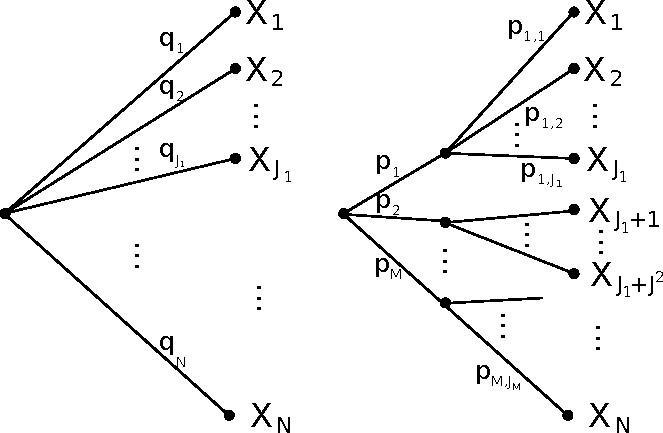
\includegraphics[width=0.5\textwidth]{images/choicesM.pdf}
        \label{fig:choicesM}
        \end{figure} 

  De forma geral, como $q_n = p_m p_{m,j}$, teremos
  \begin{eqnarray}
  H(X) &=& - \sum_{n=1}^N q_n \log q_n = - \sum_{m=1}^M \sum_{j=1}^{J_m} p_m p_{m,j} \log p_m p_{m,j} \nonumber \\
        &=& - \sum_{m=1}^M \sum_{j=1}^{J_m} \left( p_m p_{m,j} \log p_m + p_m p_{m,j} \log p_{m,j} \right) \nonumber \\
        &=& - \sum_{m=1}^M \sum_{j=1}^{J_m} p_m p_{m,j} \log p_m - \sum_{m=1}^M \sum_{j=1}^{J_m} p_m p_{m,j} \log p_{m,j} \nonumber \\
        &=& - \sum_{m=1}^M p_m \log p_m \left( \sum_{j=1}^{J_m} p_{m,j} \right) - \sum_{m=1}^M p_m \sum_{j=1}^{J_m} p_{m,j} \log p_{m,j} \nonumber \\
        &=& H(p_1, \ldots, p_M) + \sum_{m=1}^M p_m H(p_{m,1}, \ldots, p_{m,J_m}) .
  \end{eqnarray}
  
\end{frame}

\subsection{Embaralhar}
\begin{frame}%[allowframebreaks]
  \frametitle{Embaralhar}
  \begin{itemize}
  \item Suponha que $X$ seja uma v.a. indicando as posições de cartas (i.e. $X=x$ representa
  um conjunto de posições, uma determinada configuração).
  \item Seja $T$ uma operação de embaralhamento independente, i.e. $T \independent X$.
  \item Então $H(TX) \geq H(X)$.
  \begin{eqnarray}
  H(TX) &\geq& H(TX|T) \nonumber \\
        && \parbox[c]{0.7\linewidth}{\small onde utilizamos que condicionar não pode aumentar a entropia, como veremos adiante} \nonumber \\
        &=& H(T^{-1}TX|T) \nonumber \\
        && \parbox[c]{0.7\linewidth}{\small como $T$ é conhecido, aplicá-lo novamente ou seu inverso não altera a entropia} \nonumber \\
        &=& H(X|T) = H(X) \\
        && \parbox[c]{0.7\linewidth}{\small onde utilizamos que $T \independent X$} \nonumber
  \end{eqnarray}

%  \begin{equation}
%  H(TX) \geq H(TX|T) = H(T^{-1}TX|T) = H(X|T) = H(X)
%  \end{equation}
%  (onde utilizamos que condicionar não pode aumentar a entropia, como veremos adiante).
  \end{itemize}
\end{frame} 

\begin{frame}%[allowframebreaks]
  \frametitle{Permutação}
  O que ocorre se permutarmos as probabilidades?
  
  Seja $p=(p_1, p_2, \ldots, p_n)$, uma distribuição discreta de probabilidade e
  $\sigma = (\sigma_1, \sigma_2, \ldots, \sigma_n)$ uma permutação de $1, 2, \ldots, n$.
  
  Considere $p_\sigma = (p_{\sigma_1}, p_{\sigma_2}, \ldots, p_{\sigma_n} )$ uma permutação
  da distribuição $p$.

  Quem será maior? $H(p)$ ou $H(p_\sigma)$?

  %\pause
  \begin{equation}
  H(p) = - \sum_i p_i \log p_i = - \sum_j p_{\sigma_j} \log p_{\sigma_j} = H(p_\sigma)  .
  \end{equation}
\end{frame}

\subsection{Sumário}
\begin{frame}%[allowframebreaks]
  \frametitle{Sumário}
  Definição de Entropia
  \begin{equation}
  H(X) = - \sum_x p(x) \log p(x)
  \end{equation}

  Entropia Conjunta
  \begin{equation}
  H(X,Y) = - \sum_{x,y} p(x,y) \log p(x,y)
  \end{equation}

  Entropia Condicional
  \begin{equation}
  H(Y|X) = - \sum_{x,y} p(x,y) \log p(y|x)
  \end{equation}

  Regra da Cadeia
  \begin{equation}
  H(X,Y) = H(X) + H(Y|X) = H(Y) + H(X|Y)
  \end{equation}

  Limites da Entropia
  \begin{equation}
  0 \leq H(X) \leq \log n , \textmd{onde } n \textmd{ é o tamanho do alfabeto de } X.
  \end{equation}

\end{frame}


\subsection{Entropia do Jogo de Adivinhação}

\begin{frame}%[allowframebreaks]
  \frametitle{Entropia do Jogo de Adivinhação}
  Qual é a melhor estratégia para adivinhar o valor de uma variável aleatória
  com perguntas sim/não do tipo ``$X\in S$?'', para algum conjunto $S \subseteq D_X$
  (domínio da v.a. $X$).

  \begin{exampleblock}{Exemplo}
    Seja $X \in D_X = \{x_1, x_2, x_3, x_4, x_5\}$ com probabilidades
        \begin{tabular}{ c | c c c c c}
          $x$    & $x_1$ & $x_2$ & $x_3$ & $x_4$ & $x_5$ \\ \hline
          $p(x)$ & 0.3   & 0.2   & 0.2   & 0.15  & 0.15 \\
        \end{tabular}

    Considere a seguinte estratégia: 
    \begin{inlineenumerate}
        \item $X = x_5$? 
        \item $X = x_4$?
        \item $X = x_3$?
        \item $X = x_2$?
        \item $X = x_1$?
    \end{inlineenumerate}

    Desta forma faremos 5 perguntas 30\% das vezes, 4 perguntas 20\% das vezes, etc.

    O número médio de perguntas é:
    $(0.3, 0.2, 0.2, 0.15, 0.15) \cdot (5,4,3,2,1)^\intercal = 3.35$.

    Se invertermos a ordem das perguntas teremos:
    $(0.3, 0.2, 0.2, 0.15, 0.15) \cdot (1,2,3,4,5)^\intercal = 2.65$.

    Existe uma estratégia melhor?
  \end{exampleblock}
\end{frame}

\begin{frame}%[allowframebreaks]
  \frametitle{Entropia do Jogo de Adivinhação}

  Considere a estratégia ilustrada abaixo.
  \begin{figure}[h!]
  \centering
  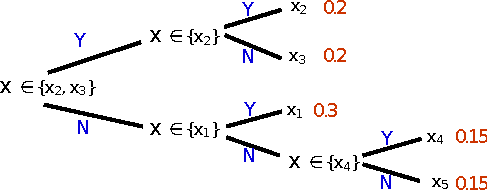
\includegraphics[width=0.75\textwidth]{images/ex-jogo-ad.pdf}
  %\caption{.}
  \label{fig:ex-jogo-ad}
  \end{figure} 

  O número médio de perguntas será:
  $2(0.2 + 0.2 + 0.3) + 3 (0.15 + 0.15) = 2.3$

  Note que $H(X) = 2.271$.

  O número médio de perguntas é sempre $\geq H(X)$.
\end{frame}

\begin{frame}%[allowframebreaks]
  \frametitle{Entropia do Jogo de Adivinhação}
  Vamos analisar a melhor e a pior estratégias, vistas anteriormente,
  com relação à forma como elas dividem a distribuição.

  \begin{itemize}
  \item pior estratégia: $X = x_5$?
 
  Divide a distribuição em dois grupos ($X=x_5$ e $X \neq x_5$), com probabilidades
  $p(X=x_5) = 0.15$, $p(X\neq x_5)=0.85$, e a entropia será $H(0.15 , 0.85) = 0.6098$.

  \item melhor estratégia: $X\in\{x_2,x_3\}$?
  
  $p(X\in\{x_2,x_3\})=0.4$, $p(X\notin\{x_2,x_3\})=0.6$, $H(0.4, 0.6)=0.971$.

  \item De forma geral, é melhor realizar primeiro perguntas que, analisadas como
  variáveis aleatórias, possuem maior entropia (algoritmo guloso).

  \item Note a relação com $H(Y|X) + H(X) = H(X,Y)$. Se fizermos uma pergunta com
  $H(X)$ grande, a entropia residual $H(Y|X)$ fica menor.
  \end{itemize}
\end{frame}
\note{
  Veremos adiante que o algoritmo guloso não é ótimo (entropia mínima).
}



